Über das eingesetzte Projektplanungstool Notion wurden die Abweichungen zwischen Soll und Ist Terminen erfasst und die Abweichungen berechnet. Das Ergebnis ist in Abbildung~\ref{Zeitplan_Soll_Ist} dargestellt.

\begin{figure}[H]
    \centering
    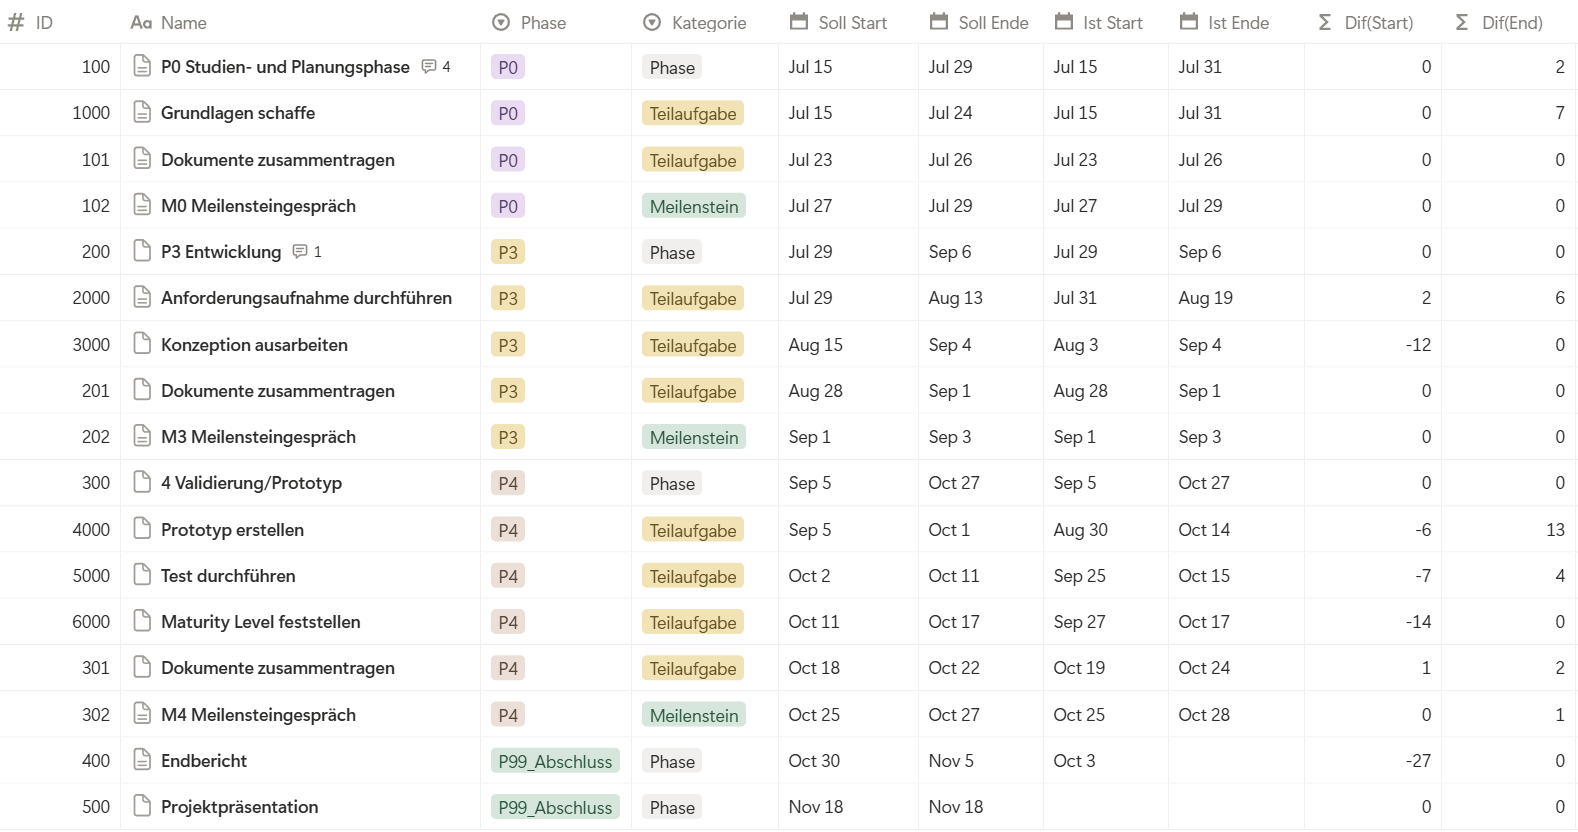
\includegraphics[width=1\textwidth]{Zeitplan_Soll_Ist.png}
    \caption{Soll/Ist-Zeitplan}\label{Zeitplan_Soll_Ist}
\end{figure}

Aus der Abbildung~\ref{Zeitplan_Soll_Ist} ist erkennbar, dass es Abweichungen gab, diese jedoch kompensiert wurden. Auffällig sind negative Abweichungen. Diese sind entstanden, da nicht alle Projektmitglieder an denselben Themen zur selben Zeit arbeiten konnten. Daher wurden in Abstimmung bereits einzelne Dokumentenstrukturen und Vorlagen für zum Beispiel Testläufe vorzeitig erstellt. Die größte Verzögerung ist bei der Teilaufgabe „Prototyp erstellen“ zu sehen. Diese ist mit bereits erwähnten Nachbesserungsbedarfen begründet. Entsprechend später konnten die Testdurchläufe durchgeführt werden. Die nächstgrößeren Verzögerungen sind bei der Teilaufgabe „Grundlage schaffen“ und „Anforderungsaufnahme durchführen“ zu sehen. Diese ist entstanden, da der erste Meilenstein M0 nur unter Auflagen bestanden wurde. Diese Auflagen wurden priorisiert bearbeitet. 